\section{Gesichtserkennung}
\label{MTCNN}
Multi-task Cascaded Convolutional Networks (MTCNN) ist ein Algorithmus zur Detektion von Gesichtern und Bestimmung von 5 Gesichts-Landmarks in Farbbildern. Es machte im Vorabtests auf Probebildern einen sehr guten Eindruck und konnte die meisten Gesichter mit verschieden Größen und Blickrichtungen finden.\\
Für die Detektion werden drei CNN auf einer Bildpyramide angewendet um zuverlässig Gesichter verschiedenster Größe zu erkennen. Außerdem wird für die Detektion der Gesichter auch deren Ausrichtung berücksichtigt, um bessere Ergebnisse zu erzielen. Laut Beschreibung des Verfahrens sollen somit sogar recht kleine Gesichter mit $20\times 20$ Pixeln erfassbar sein.\\
Sein Einsatzgebiet in der aktuellen Anwendung ist die Vorverarbeitung eines Frames für die spätere Auswertung. Somit soll dieser Schritt von einem möglichst robusten Verfahren durchgeführt werden. Dabei wird im aktuellen Fall auf einem hochauflösenden Bild gearbeitet mit verhältnismäßig kleinen, verschieden großen und weit verteilten Gesichtern.
\subsection{Die 3 Stufen der Verarbeitung}
Für die gute Detektionsqualität sorgt die dreistufige Verarbeitung mit verschiedenen CNN auf einer Bildpyramide. Bei der Bildpyramide handelt es sich um ein in verschiedenen Größen skaliertes Bild, damit der gesuchte Inhalt in der gewünschten Auflösung abgebildet ist, ohne etwas über den Inhalt zu wissen.\\
Dies ist von Vorteil, damit das CNN auf eine feste Größe von Gesichtern optimiert werden kann, um das Lernen nicht zusätzlich zu erschweren. So werden nur die Farbverläufe gelernt und nicht weiter durch die Skalierung erschwert, wodurch das CNN auf seine jeweilige Aufgabe besser optimiert werden kann.
\begin{figure}
	\centering
	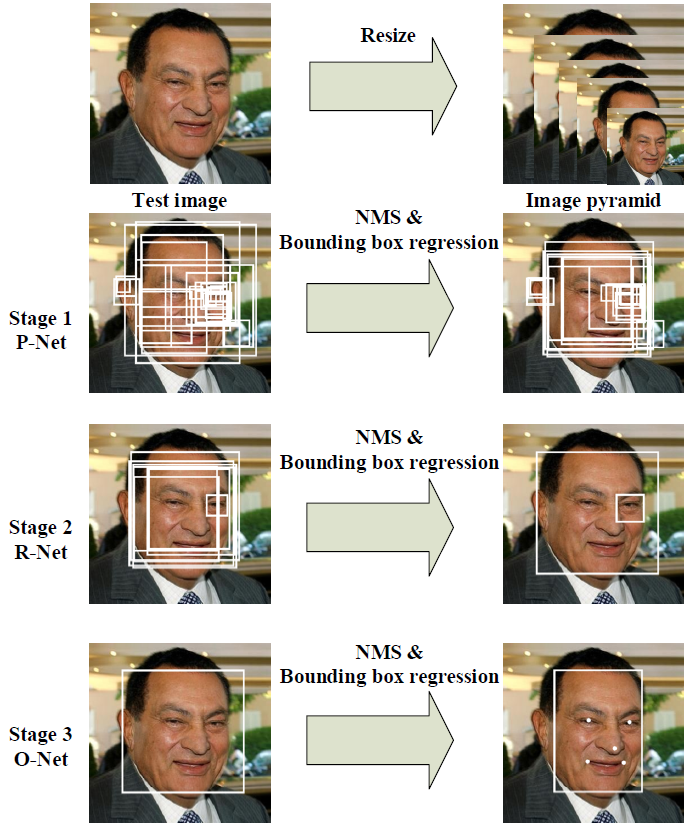
\includegraphics[width=0.5\linewidth]{img/MTCNN_Step}
	\caption{Darstellung des Funktionsablaufes von MTCNN, Abbildung aus \cite{MTCCN}}
	\label{img_MTCNN_Step}
\end{figure}
\subsubsection{Stufe 1}
Beim ersten Verarbeitungsschritt werden alle Bereiche eines Bilds gesucht, in denen möglicherweise ein Gesicht zu erkennen ist. Dazu wird für die Detektion ein CNN eingesetzt, dem sogenannten Proposal Network (P-Net), das alle möglichen Bounding-Boxen ermittelt in denen ein Gesicht zu sehen sein könnte. Diese Bounding-Boxen werden anschließend mit einem NMS ausgedünnt, um die am stärksten überlappenden Boxen zusammen zu fassen. Dies ist notwendig, da dieses CNN zwar recht schnell arbeitet, allerdings auch mit einer sehr großen False-True-Fehlerrate (Erkennen trotz nicht vorhanden).
\subsubsection{Stufe 2}
Die möglichen Bereiche aus Stufe 1 werden anschließend mittels eines weiteren CNN analysiert, damit alle Nicht-Gesichtsbereiche erkannt und entfernt werden können. Dies wird von dem Refine Network (R-Net) übernommen und anschließend die möglichen Bounding-Boxen mittels NMS noch weiter reduziert.
\subsubsection{Stufe 3}
Der letzte Schritt wird von einem deutlich genaueren CNN übernommen, um ein Gesicht zu detektieren, dem sogenannten Output Network (O-Net). Womit die resultierenden exakten Boxen mit ihren jeweiligen 5 Landmarks ermittelt werden.
\subsection{Zuverlässigkeit bei der Detektion}
MTCNN Face Detection ist bei der Zuverlässigkeit im Verglich zu anderen bekannten Verfahren laut ihrem Paper \cite{MTCCN} überlegen. Zudem auf $640\times 480$ großen Bildern echtzeitfähig und kann vor allem auch sehr kleine Gesichter erfolgreich erkennen.\\
Somit sind alle Anforderungen erfüllt um mit diesem Verfahren den vorhanden Frame für die nachfolgenden Berechnungen vorzubereiten. Ein Test bestätigt diese Annahme, siehe \autoref{img_bereich_MTCNN}.
Die 5 bestimmten Landmarks von MTCNN-Face sind allerdings gerade bei sehr kleinen Bildbereichen zu ungenau und deshalb im Folgenden nicht weiter verwendbar.
